\documentclass[10pt,journal,compsoc]{IEEEtran}

\input{math_commands.tex}

\usepackage[utf8]{inputenc}
\usepackage{amsmath}
\usepackage{amssymb}
\usepackage{amsthm}
\newtheorem{prop}{Proposition}
\usepackage{booktabs}
\usepackage{graphicx}
\usepackage[hidelinks]{hyperref}
\usepackage{url}
\usepackage{tikz}
\usepackage{cite}
\usepackage{geometry}
\geometry{letterpaper, margin=0.75in}
\usetikzlibrary{shadows, arrows.meta, positioning, fit, backgrounds, shapes.geometric, arrows}

\newcommand{\reqexp}[1]{\noindent\textbf{[REQUIRED EXPERIMENT --- #1]}}
\newcommand{\refneeded}[1]{\textbf{[REFERENCE NEEDED: #1]}}
\newcommand{\authconfirm}[1]{\textbf{[AUTHOR MUST CONFIRM: #1]}}

\definecolor{orcidlogocolor}{HTML}{A6CE39}
\DeclareRobustCommand{\orcidicon}[1]{\href{https://orcid.org/#1}{\mbox{\scalebox{0.75}{\tikz[baseline=-0.4ex]{
  \fill[orcidlogocolor] (0,0) circle (0.52em);
  \node[color=white,font=\sffamily\bfseries] at (0,0) {\fontsize{4.5pt}{4.5pt}\selectfont iD};
}}}}}

\begin{document}

\markboth{Journal of Computer Science \& Technology (JCS\&T),~Vol.~XX,~No.~X,~2026}%
{Akhyar: Delta BPTT: Efficient Add-Only Backpropagation Through Time}

\twocolumn[{%
  \begin{center}
    {\small -- ORIGINAL ARTICLE --} \\[0.8em]

    {\Huge\bfseries Delta BPTT: Event-Gated Backpropagation Through Time for Efficient Spiking Sequence Representations} \\[0.6em]

    {\large\bfseries Delta BPTT: Retropropagación a Través del Tiempo Regulada por Eventos para Representaciones Eficientes de Secuencias con Impulsos Neurales} \\[1.0em]

    {\fontsize{11pt}{13pt}\selectfont Muhammad Akhyar$^{1}$\,\orcidicon{0009-0001-3259-4996}} \\[0.8em]

    {$^{1}$\emph{Independent Researcher}} \\
    \emph{akhyarsafrudin@gmail.com} \\[1.2em]
  \end{center}

  \noindent
  \begin{minipage}[t]{0.48\linewidth}
    {\large\bfseries Abstract}\\[0.4em]
    {\fontsize{8.5pt}{10.2pt}\selectfont Spiking Neural Networks (SNNs) offer an event-driven alternative to conventional deep networks by replacing dense floating-point multiplications with sparse accumulations. When SNNs are trained with Backpropagation Through Time (BPTT), however, parameter-gradient accumulation traditionally retains dense Multiply--Accumulate (MAC) operations. In this paper, we present \textbf{Delta BPTT}, an event-gated execution formulation of BPTT for binary spike representations in which input spikes gate weight-vector accumulation, turning both forward recurrent projections and weight-gradient updates into conditional vector additions. Evaluated on a $65$K-trainable-parameter recurrent pooler attached to a frozen static embedding table across the ALL-STS teacher-fidelity aggregate and STS-B benchmarks ($29{,}720$ sentence pairs), Delta BPTT eliminates spike-gated MACs ($67.2\%$ activity sparsity matching the forward pass) and accelerates CPU training by $2.44\times$ over Standard BPTT with a gradient cosine similarity of $0.9982$. Furthermore, the recurrent embedder architecture reduces CPU training time by $4.13\times$ compared to Spike-Overlap attention while maintaining high correlation fidelity. An operation-based 45\,nm energy proxy suggests a whole-pooler energy reduction of $\approx 2.7\times$ (up to $15.6\times$ for the isolated spike-gated weight update).}

    \vspace{0.6em}
    {\fontsize{8.5pt}{10.2pt}\selectfont\textbf{Index Terms---}Spiking Neural Networks, Backpropagation Through Time, Sequence Representation, Sentence Embeddings, Neuromorphic Computing, Delta BPTT.}
  \end{minipage}%
  \hfill
  \begin{minipage}[t]{0.48\linewidth}
    {\large\bfseries Resumen}\\[0.4em]
    {\fontsize{8.5pt}{10.2pt}\selectfont Las Redes Neuronales de Impulsos (SNNs) ofrecen una alternativa por eventos frente a las redes profundas al sustituir multiplicaciones en coma flotante por acumulaciones dispersas. Sin embargo, el entrenamiento con Retropropagación a Través del Tiempo (BPTT) mantiene operaciones densas de Multiplicación y Acumulación (MAC) durante la acumulación de gradientes. En este artículo presentamos \textbf{Delta BPTT}, una formulación de ejecución regulada por eventos para impulsos binarios donde los impulsos de entrada controlan la acumulación de vectores de pesos, convirtiendo las proyecciones y actualizaciones de gradientes en sumas vectoriales condicionales. Evaluado en un agrupador recurrente de $65$K parámetros entrenables acoplado a una tabla de embebidos estáticos congelados en las pruebas ALL-STS y STS-B ($29.720$ pares de oraciones), Delta BPTT elimina las operaciones MAC reguladas por impulsos ($67{,}2\%$ de dispersión) y acelera el entrenamiento en CPU en $2{,}44\times$ frente a BPTT Estándar con una similitud coseno de gradientes de $0{,}9982$. Asimismo, la arquitectura del agrupador recurrente reduce el tiempo de entrenamiento en $4{,}13\times$ respecto a la atención Spike-Overlap. Una estimación energética a 45\,nm sugiere una reducción de energía del agrupador completo de $\approx 2,7\times$ (hasta $15{,}6\times$ para el término de actualización de pesos regulado por impulsos).}

    \vspace{0.6em}
    {\fontsize{8.5pt}{10.2pt}\selectfont\textbf{Palabras clave---}Redes Neuronales de Impulsos, Retropropagación a Través del Tiempo, Representación de Secuencias, Embebidos de Oraciones, Computación Neuromórfica, Delta BPTT.}
  \end{minipage}
  \vspace{1.0em}
}]

\section{Introduction}

The computational overhead of dense sentence embedders \cite{devlin2018bert}, such as SBERT \cite{reimers2019sentence}, is dominated by the matrix multiplications of scaled dot-product attention \cite{vaswani2017attention}. While numerous efficient Transformer variants mitigate this quadratic $\mathcal{O}(L^2)$ cost \cite{tay2022efficient}, they continue to rely on continuous floating-point arithmetic. Spiking Neural Networks (SNNs) take a different route: because their activations are binary spike events, synaptic integration can in principle be executed as sparse, event-driven accumulation rather than dense multiplication, which makes SNNs attractive for neuromorphic hardware \cite{roy2019towards}. Recent neuromorphic NLP research has ported self-attention into the spiking domain \cite{li2022spikeformer, zhu2023spikegpt}, and frameworks such as SpikingJelly \cite{fang2023spikingjelly} have accelerated the validation of surrogate-gradient training in deep spiking architectures.

A frequently overlooked bottleneck, however, lies not in the \emph{forward} pass---where spike-driven sparsity is well established---but in the \emph{backward} pass. Standard BPTT with surrogate gradients \cite{neftci2019surrogate} propagates continuous error signals backward through the unrolled network, and the weight-gradient accumulation $\Delta\mW = \sum_t \bm{\delta}^{(t)} (\mX^{(t)})^T$ is conventionally evaluated as a dense outer product even when $\mX^{(t)}$ is a binary spike vector. This is mathematically unnecessary: when the gating signal is strictly binary, the outer product degenerates into a selection of rows, and selection can be executed as conditional accumulation. Existing SNN training formulations do not expose this structure as an explicit event-driven execution rule with a precise operation accounting. This raises two questions: \textit{(1)~Can the spike-gated phases of BPTT---the forward projection and the weight-gradient accumulation---be executed as conditional additions, and what exactly is saved? (2)~Are explicit spatial attention mechanisms necessary for sentence-level representation, or does native temporal recurrence paired with such a learning rule suffice?}

We address both questions with \textbf{Delta BPTT}, an event-gated recurrent training rule. The central observation is algebraic: for a binary vector $\mS^{(t)} \in \{0,1\}^{D_{in}}$, the identity $\mW^T \mS^{(t)} = \sum_{d:\,S^{(t)}_d = 1} \mW_{d,:}$ is exact, and the right-hand side contains no multiplication. The same identity applies to the gradient outer product $\sum_t \mS^{(t)}(\tilde{\bm{\delta}}^{(t)})^T$. Delta BPTT executes both phases by iterating over active spike events only. We emphasize the scope of this claim throughout: multiplications inside the neuron dynamics, the temporal error recurrence, the surrogate-gradient mask, and the error back-projection to earlier layers are \emph{not} removed. Our empirical findings indicate that the recurrent pooler trained with this rule is sufficient for encoding semantic structure in the sentence-embedding setting, reaching $93.5\%$ of the STS-B Spearman correlation of SpikingBERT \cite{bal2024spikingbert} with $770\times$ fewer parameters and no GPU.

\subsection{Contributions}
\begin{itemize}
    \item \textbf{Event-Gated Execution Rule.} We introduce Delta BPTT, an event-gated execution rule for binary spike representations that converts both forward recurrent weight projections and backward weight-gradient updates into conditional vector additions, bypassing dense outer products without modifying the underlying learning objective.
    \item \textbf{Exact Algebraic Equivalence \& Operation Accounting.} We prove that Delta BPTT is algebraically equivalent to Standard BPTT in exact arithmetic ($\Theta(L D_{in} D_{out})$ complexity with active work $a L D_{in} D_{out}$ ACs at spike activity rate $a$), and delimit precisely which operations are converted (spike-gated MACs) versus retained (neuron dynamics, error back-projection).
    \item \textbf{Empirical Validation on Sequence Representations.} We validate Delta BPTT on semantic sentence embedding benchmarks (STS-12--16, STS-B, SICK-R), demonstrating that our 65K trainable parameter pooler recovers $88.3\%$ of the teacher's zero-shot performance, yields a $2.44\times$ CPU training speedup over dense BPTT ($4.13\times$ over attention baselines), and aligns with Standard BPTT gradients ($\cos = 0.9982$, relative error $0.34\%$).
\end{itemize}

\section{Related Work}

\subsection{Spiking Neural Networks for Language}
Recent work has ported Transformer primitives into the spiking domain. SpikFormer \cite{zhou2023spikformer} introduced spike-driven self-attention for vision, and SpikeGPT \cite{zhu2023spikegpt} scaled spiking architectures to generative language modeling with up to 216M parameters. For encoder-style representations, SpikeBERT \cite{lv2023spikebert} applies two-stage knowledge distillation from BERT, while SpikingBERT \cite{bal2024spikingbert} integrates spiking neurons with BERT-style pretraining and reports GLUE results---including a Spearman correlation of $0.819$ on STS-B---with approximately $50$M parameters; Spikingformer \cite{zhou2025spikingformer} stabilizes spike-driven residual learning and reports $0.545$ on STS-B with $66$M parameters. Two observations motivate our study. First, these models retain an explicit $\mathcal{O}(L^2)$ attention mechanism that dominates their operation counts. Second, none of them targets \emph{sentence embeddings} or reports the standard STS suite (STS-12 through STS-16, STS-B, SICK-R) against human judgments; to the best of our knowledge, our $65$K-parameter recurrent pooler is among the first SNNs evaluated directly on this suite, though we do not claim absolute priority.

\subsection{Efficient Sentence Embedding}
Dense sentence embedders are typically obtained by fine-tuning pretrained encoders with siamese \cite{reimers2019sentence} or contrastive objectives \cite{gao2021simcse}, and compressed via knowledge distillation \cite{hinton2015distilling, sanh2019distilbert, wang2020minilm} or quantization. These models define the accuracy frontier---DistilBERT reports $0.869$ Spearman on STS-B \cite{sanh2019distilbert}---but rely on continuous floating-point matrix multiplications. Static embeddings with mean pooling (Word2Vec, GloVe) remain competitive low-cost baselines and are included in our evaluation. The standard evaluation convention for this task family is correlation against human gold labels \cite{muennighoff2022mteb, cer2017semeval}, which we adopt for the zero-shot track of our evaluation.

\subsection{Temporal Credit Assignment and Event-Driven Training}
Surrogate-gradient BPTT \cite{neftci2019surrogate} is the dominant training method for deep SNNs, but its backward pass is dense in time and in space. Alternatives include truncated BPTT, eligibility-propagation rules (e-prop) \cite{bellec2020solution}, event-driven gradient methods for continuous-time spiking dynamics (e.g., EventProp) \cite{wunderlich2021event}, and online approximations such as real-time recurrent learning; sparse matrix--vector kernels form the classical computing counterpart of spike-gated accumulation \cite{zenke2021remarkable}. Delta BPTT is orthogonal to these methods: it does not approximate or truncate the temporal credit assignment---the recurrence is identical to Standard BPTT---but changes the \emph{execution} of the spike-gated operations from dense multiplication to conditional accumulation. To our knowledge, existing SNN training pipelines do not state this execution rule and its operation accounting explicitly.

\subsection{Energy Accounting for SNNs}
SNN efficiency claims conventionally rely on operation counting: spike-driven accumulate operations (SOPs/ACs) are contrasted with multiply--accumulate operations (MACs), weighted by the 45\,nm energy figures of Horowitz \cite{horowitz2014computing} ($0.9$\,pJ per 32-bit accumulation versus $4.6$\,pJ per 32-bit MAC) \cite{zhou2023spikformer, fang2023spikingjelly}. This proxy omits memory access and data movement, which can dominate real energy budgets. Moreover, existing analyses focus on the \textit{forward} pass; the backward pass of BPTT is tacitly assumed to require dense MACs throughout. We therefore report the theoretical proxy and measured CPU latency side by side and treat the proxy strictly as an upper-bound estimate, never as a hardware measurement.

\section{Methodology: Delta BPTT and Architectural Dynamics}

\begin{figure}[t!]
\begin{center}
\resizebox{0.95\linewidth}{!}{%
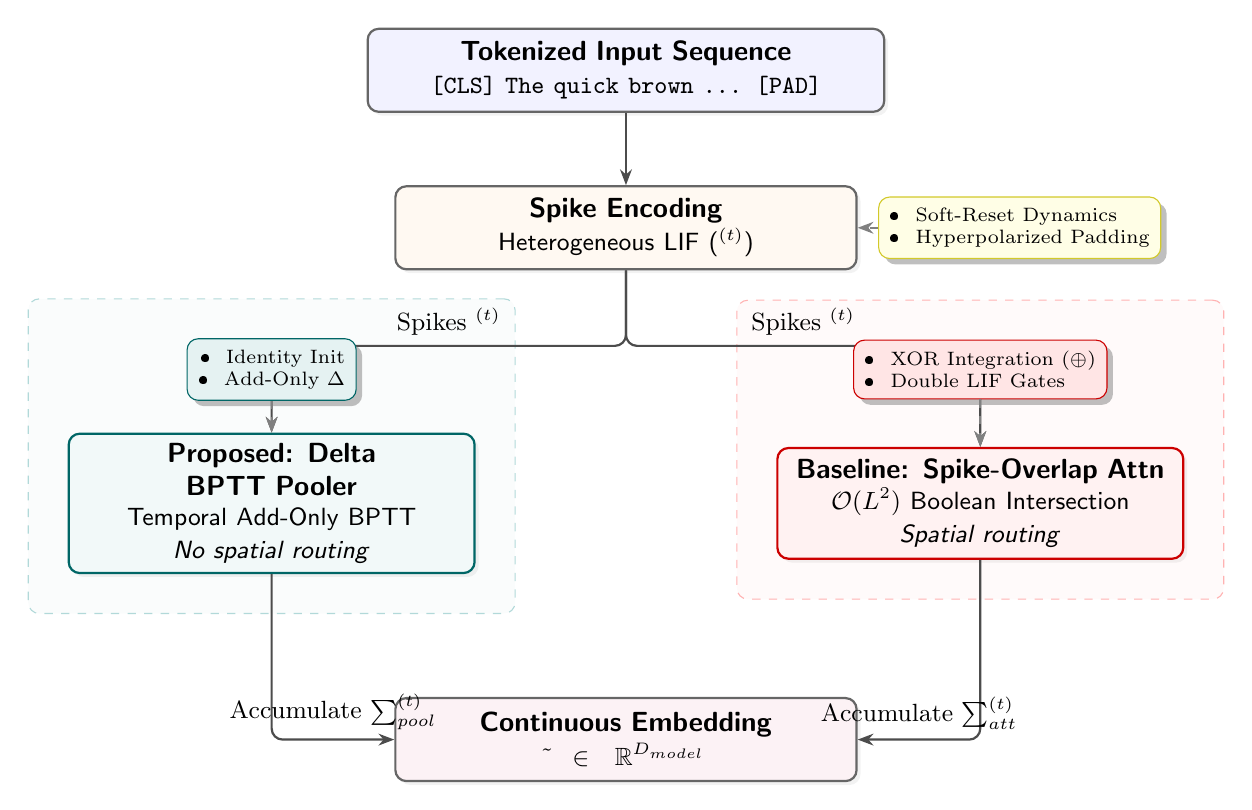
\begin{tikzpicture}[
    font=\sffamily,
    base/.style={rectangle, rounded corners, draw=black!60, thick, minimum height=3em, align=center, fill=white, drop shadow={opacity=0.1, shadow xshift=0.05cm, shadow yshift=-0.05cm}},
    input/.style={base, fill=blue!5, text width=18em},
    spike/.style={base, fill=orange!5, text width=16em},
    pooler/.style={base, fill=teal!5, text width=14em, minimum height=4em, draw=teal!80!black},
    attn/.style={base, fill=red!5, text width=14em, minimum height=4em, draw=red!80!black},
    output/.style={base, fill=purple!5, text width=16em},
    arrow/.style={-{Stealth[length=2mm]}, thick, draw=black!70},
    dashed_arrow/.style={-{Stealth[length=2mm]}, dashed, thick, draw=black!50}
]

% Center column
\node[input] (tokens) at (0, 0) {\textbf{Tokenized Input Sequence} \\ \small \texttt{[CLS] The quick brown ... [PAD]}};
\node[spike] (lif) at (0, -2) {\textbf{Spike Encoding} \\ \small Heterogeneous LIF ($\mV^{(t)}$)};
\draw[arrow] (tokens) -- (lif);

% Left branch (Proposed)
\node[pooler] (recurrent) at (-4.5, -5.5) {\textbf{Proposed: Delta BPTT Pooler} \\ \small Temporal Add-Only BPTT \\ \small \textit{No spatial routing}};

% Right branch (Baseline)
\node[attn] (attention) at (4.5, -5.5) {\textbf{Baseline: Spike-Overlap Attn} \\ \small $\mathcal{O}(L^2)$ Boolean Intersection \\ \small \textit{Spatial routing}};

% Split paths
\draw[arrow, rounded corners] (lif) -- (0, -3.5) -| node[above, pos=0.25, font=\small, text=black] {Spikes $\mS^{(t)}$} (recurrent);
\draw[arrow, rounded corners] (lif) -- (0, -3.5) -| node[above, pos=0.25, font=\small, text=black] {Spikes $\mS^{(t)}$} (attention);

% Output
\node[output] (out) at (0, -8.5) {\textbf{Continuous Embedding} \\ \small $\tilde{\mE} \in \mathbb{R}^{D_{model}}$};

% Join paths
\draw[arrow, rounded corners] (recurrent) |- node[above, pos=0.75, font=\small, text=black] {Accumulate $\sum \mV_{pool}^{(t)}$} (out);
\draw[arrow, rounded corners] (attention) |- node[above, pos=0.75, font=\small, text=black] {Accumulate $\sum \mV_{att}^{(t)}$} (out);

% Annotations
\node[align=left, font=\scriptsize, text=black, fill=yellow!10, draw=yellow!80!black, rounded corners, inner sep=4pt, drop shadow] (note1) at (5, -2) {\textbullet~ Soft-Reset Dynamics \\ \textbullet~ Hyperpolarized Padding};
\draw[dashed_arrow] (note1) -- (lif);

\node[align=right, font=\scriptsize, text=black, fill=teal!10, draw=teal!80!black, rounded corners, inner sep=4pt, drop shadow] (note2) at (-4.5, -3.8) {\textbullet~ Identity Init \\ \textbullet~ Add-Only $\Delta\mW$};
\draw[dashed_arrow] (note2) -- (recurrent);

\node[align=left, font=\scriptsize, text=black, fill=red!10, draw=red!80!black, rounded corners, inner sep=4pt, drop shadow] (note3) at (4.5, -3.8) {\textbullet~ XOR Integration ($\oplus$) \\ \textbullet~ Double LIF Gates};
\draw[dashed_arrow] (note3) -- (attention);

% Background groupings
\begin{scope}[on background layer]
    \node[fill=teal!2, rounded corners, draw=teal!30, dashed, inner sep=0.5cm, fit=(recurrent) (note2)] {};
    \node[fill=red!2, rounded corners, draw=red!30, dashed, inner sep=0.5cm, fit=(attention) (note3)] {};
\end{scope}

\end{tikzpicture}%
}
\end{center}
\caption{Architectural flowchart contrasting the proposed Delta BPTT Recurrent Pooler (core contribution) against the $\mathcal{O}(L^2)$ Spike-Overlap Attention baseline (secondary, ablation-only component).}
\label{fig:architecture}
\end{figure}

Our spiking sentence embedder constructs continuous semantic representations from discrete spike events. The pipeline consists of spike encoding, a sequence aggregation mechanism (the proposed recurrent pooler, or the attention baseline), and knowledge-distillation training. Table~\ref{tab:notation} fixes the notation used throughout.

\begin{table}[t!]
\caption{Notation used throughout the paper.}
\label{tab:notation}
\begin{center}
\resizebox{\linewidth}{!}{%
\begin{tabular}{ll}
\toprule
\textbf{Symbol} & \textbf{Meaning} \\
\midrule
$L$ (=$T$) & sequence length in tokens $=$ discrete timesteps \\
$D_{in}, D_{out}$ & pooler input / output dimension \\
$D$ & shorthand when $D_{in}=D_{out}=D$ \\
$a \in [0,1]$ & spike \emph{activity} rate (fraction of entries $=1$) \\
$s = 1-a$ & spike \emph{sparsity} ($s \approx 0.672$ measured, $a \approx 0.328$) \\
$\mS_{emb}^{(t)} \in \{0,1\}^{D_{in}}$ & embedding-layer spike vector at step $t$ \\
$\mV^{(t)}, \mU^{(t)}$ & membrane potential, pre-reset potential \\
$\bm{\beta}, \bm{\theta}$ & per-neuron leak decay and threshold (heterogeneous) \\
$\mW \in \mathbb{R}^{D_{in}\times D_{out}}$ & pooler weight matrix; $\mW_{d,:}$ its $d$-th row \\
$\tilde{\bm{\delta}}^{(t)} \in \mathbb{R}^{D_{out}}$ & masked temporal error at step $t$ \\
$\sigma'(\cdot)$ & rectangular surrogate-gradient mask (window $\gamma$) \\
$E, \tilde{\mE}$ & sentence embedding and its $\ell_2$ normalization \\
\bottomrule
\end{tabular}%
}
\end{center}
\end{table}

\subsection{Spike Encoding and Heterogeneous Dynamics}
Raw text is tokenized (BPE; vocabulary file loaded at runtime) into indices $\vx^{(1:L)}$. A spiking embedding layer maps each token to a temporal spike train; the temporal dimension coincides with the sequence dimension, i.e., token position $t$ \emph{is} timestep $t$. Writing $\mW_{emb}[\vx^{(t)}] \in \mathbb{R}^{D_{in}}$ for the embedding row of token $\vx^{(t)}$ (equivalently, a matrix product with a one-hot vector), the membrane dynamics follow a Leaky Integrate-and-Fire (LIF) model with soft reset:
\begin{align}
\mU_{emb}^{(t)} &= \min\!\left(1.0,\; \bm{\beta}_{emb} \odot \mV_{emb}^{(t-1)} + \mW_{emb}[\vx^{(t)}]\right), \label{eq:lif_u}\\
\mS_{emb}^{(t)} &= H\!\left(\mU_{emb}^{(t)} - \bm{\theta}_{emb}\right) \in \{0,1\}^{D_{in}}, \label{eq:lif_s}\\
\mV_{emb}^{(t)} &= \mU_{emb}^{(t)} - \mS_{emb}^{(t)} \odot \bm{\theta}_{emb}, \label{eq:lif_v}
\end{align}
where $H(\cdot)$ is the element-wise Heaviside step function and the $\min(1.0,\cdot)$ clamp bounds the pre-reset potential. We use a \emph{soft reset} (subtracting the threshold) rather than a hard reset to zero, preserving fractional sub-threshold residue across time. Leak decays and thresholds are heterogeneous across dimensions: $\beta_i = 1 - 2^{-k_i}$ with $k_i$ sampled uniformly from $\{2,\dots,7\}$ (i.e., $\beta_i \in [0.75, 0.9922]$), forcing multi-timescale temporal processing at ingestion. These element-wise operations ($\bm{\beta}\odot\mV$, the clamp, the comparison, the reset subtraction) are part of the computation that Delta BPTT does \emph{not} remove; they appear in both the Standard and Delta variants.

\textbf{Sequence Padding and Hyperpolarization.} To handle variable sequence lengths without attention masks, the embedding row of the \texttt{<PAD>} token (index $0$) is overridden to $-1.0$ in every dimension. Padding steps therefore inject a strongly negative current, hyperpolarizing the membrane ($U < 0$), which guarantees that padding emits exactly zero spikes and contributes no noise to temporal pooling.

\subsection{Ablation Baseline: Spike-Driven Spike-Overlap Attention}
To isolate the contribution of spatial routing, we formalize a spike-driven self-attention mechanism used \emph{only} as an ablation baseline; it is not part of the Delta BPTT contribution. Embedding spikes $\mS_{emb}$ are projected into Query, Key, and Value spike trains by independent LIF layers. For query token $i$ and key token $j$, the raw affinity is a Boolean match count:
\begin{equation}
M_{i,j}^{(t)} = \sum_{d=1}^{D_{model}} \left( Q_{i,d}^{(t)} \wedge K_{j,d}^{(t)} \right),
\end{equation}
normalized by $\max_k (M_{i,k}^{(t)} + \epsilon)$. The normalized scores drive an auxiliary LIF layer that emits attention-mask spikes $\mS_{scores}$, which gate the Value spikes by accumulation. Contextual features are then combined with the original embedding spikes through an exclusive-OR:
\begin{equation}
\mS_{agg}^{(t)} = \mS_{emb}^{(t)} \oplus \mS_{att}^{(t)}.
\end{equation}
The pairwise match counts cost $\mathcal{O}(L^2 \cdot D)$ per sequence (plus $\mathcal{O}(L \cdot D^2)$ for the Q/K/V projections), which is precisely the quadratic routing cost the recurrent pooler avoids.

\begin{figure}[t!]
\begin{center}
\resizebox{0.85\linewidth}{!}{%
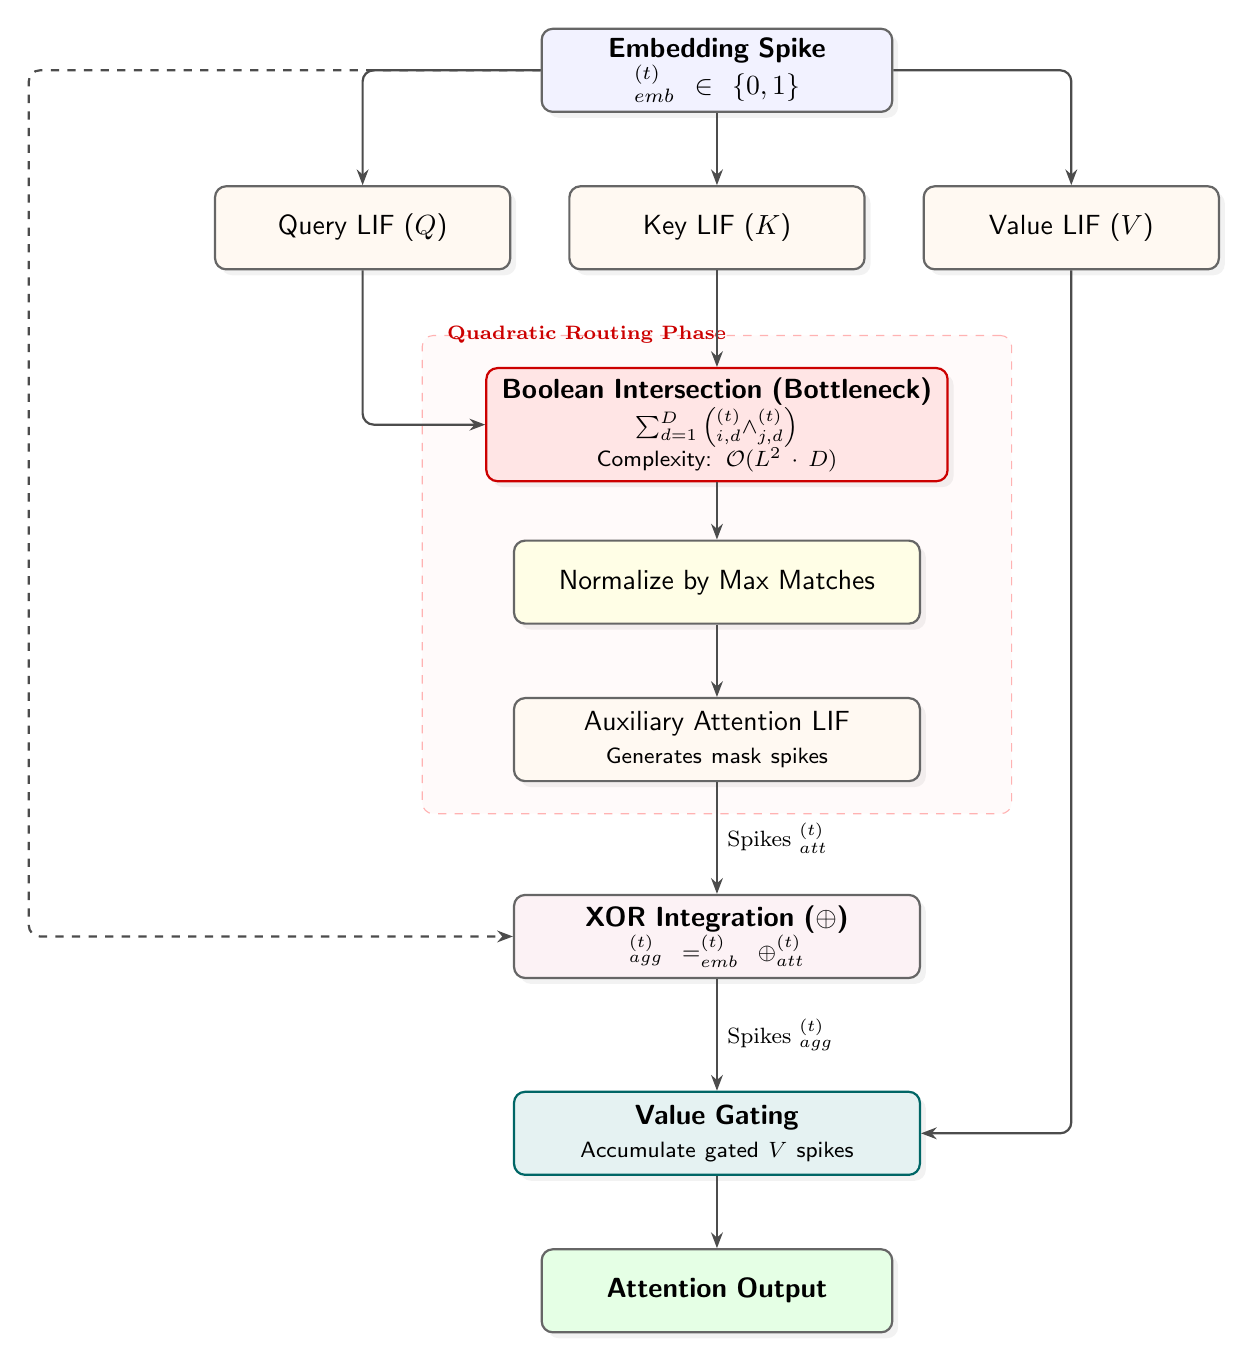
\begin{tikzpicture}[
    font=\sffamily,
    base/.style={rectangle, rounded corners, draw=black!60, thick, minimum height=3em, align=center, fill=white, drop shadow={opacity=0.1}},
    input/.style={base, fill=blue!5, text width=12em},
    proj/.style={base, fill=orange!5, text width=10em},
    compute/.style={base, fill=red!10, draw=red!80!black, text width=16em},
    gate/.style={base, fill=purple!5, text width=14em},
    arrow/.style={-{Stealth[length=2mm]}, thick, draw=black!70}
]

\node[input] (semb) at (0, 0) {\textbf{Embedding Spike} \\ $\mS_{emb}^{(t)} \in \{0,1\}$};
\node[proj] (k) at (0, -2) {Key LIF ($K$)};
\node[proj] (q) at (-4.5, -2) {Query LIF ($Q$)};
\node[proj] (v) at (4.5, -2) {Value LIF ($V$)};

\draw[arrow] (semb) -- (k);
\draw[arrow, rounded corners] (semb) -| (q);
\draw[arrow, rounded corners] (semb) -| (v);

\node[compute] (intersect) at (0, -4.5) {\textbf{Boolean Intersection (Bottleneck)} \\ \footnotesize $\sum_{d=1}^{D} \left( \mQ_{i,d}^{(t)} \wedge \mK_{j,d}^{(t)} \right)$ \\ \footnotesize Complexity: $\mathcal{O}(L^2 \cdot D)$};
\draw[arrow, rounded corners] (q) |- (intersect);
\draw[arrow] (k) -- (intersect);

\node[base, fill=yellow!10, text width=14em] (norm) at (0, -6.5) {Normalize by Max Matches};
\draw[arrow] (intersect) -- (norm);

\node[proj, text width=14em] (aux) at (0, -8.5) {Auxiliary Attention LIF \\ \footnotesize Generates mask spikes};
\draw[arrow] (norm) -- (aux);

\node[gate] (xor) at (0, -11) {\textbf{XOR Integration ($\oplus$)} \\ \footnotesize $\mS_{agg}^{(t)} = \mS_{emb}^{(t)} \oplus \mS_{att}^{(t)}$};
\draw[arrow] (aux) -- node[right, font=\footnotesize] {Spikes $\mS_{att}^{(t)}$} (xor);
\draw[arrow, rounded corners, dashed] (semb.west) -- ++(-6.5,0) |- (xor.west);

\node[gate, fill=teal!10, draw=teal!80!black] (gate_node) at (0, -13.5) {\textbf{Value Gating} \\ \footnotesize Accumulate gated $V$ spikes};
\draw[arrow] (xor) -- node[right, font=\footnotesize] {Spikes $\mS_{agg}^{(t)}$} (gate_node);
\draw[arrow, rounded corners] (v.south) |- (gate_node.east);

\node[input, fill=green!10] (out) at (0, -15.5) {\textbf{Attention Output}};
\draw[arrow] (gate_node) -- (out);

\begin{scope}[on background layer]
    \node[fill=red!2, rounded corners, draw=red!30, dashed, inner xsep=0.8cm, inner ysep=0.4cm, fit=(intersect) (norm) (aux)] (bg_attn) {};
    \node[right=0.2cm of bg_attn.north west, font=\scriptsize\bfseries, text=red!80!black] {Quadratic Routing Phase};
\end{scope}

\end{tikzpicture}%
}
\end{center}
\caption{Detailed computational flow of the Spike-Overlap Attention baseline at a single timestep (ablation-only component).}
\label{fig:attention_mech}
\end{figure}
To isolate the benefit of temporal pooling from the cost of spatial attention, we construct a Spike-Driven Spike-Overlap Attention baseline. For query $\mQ^{(t)}$, key $\mK^{(t')}$, and value $\mV^{(t')}$ spike trains, the affinity matrix is computed via bitwise AND (spike overlap) rather than floating-point dot products:
\begin{equation}
A_{t, t'} = \sum_{d=1}^{D} Q_d^{(t)} \wedge K_d^{(t')}.
\label{eq:spike_overlap}
\end{equation}
The attention map is normalized via softmax and applied to $\mV^{(t')}$. Crucially, storing and contracting the $L \times L$ affinity matrix $A$ requires $\mathcal{O}(L^2 D)$ operations per sequence and $\mathcal{O}(L^2)$ memory per head, creating a spatial routing bottleneck that scales quadratically with sequence length $L$.

\subsection{The Delta BPTT Execution Rule}
We now present the core contribution: an event-gated execution formulation that eliminates Multiply--Accumulate (MAC) operations from the two spike-gated phases of BPTT.

\textbf{Mathematical foundation.} Consider a dense weight matrix $\mW \in \mathbb{R}^{D_{in} \times D_{out}}$ and a binary spike vector $\mS \in \{0, 1\}^{D_{in}}$. The matrix-vector product $\mW^T \mS$ evaluates as:
\begin{prop}[Spike-Gated Row Accumulation]
For $\mW \in \mathbb{R}^{D_{in} \times D_{out}}$ and $\mS \in \{0, 1\}^{D_{in}}$,
\begin{equation}
\mW^T \mS \;=\; \sum_{d=1}^{D_{in}} \mW_{d,:}\, S_d \;=\; \sum_{d:\, S_d = 1} \mW_{d,:},
\end{equation}
where the last expression contains no multiplication. The identity is exact in real arithmetic; in floating point it differs from dense evaluation only by the order of summation.
\end{prop}

\noindent The forward projection is therefore executed by iterating over active spikes:
\begin{equation}
\mX_{pool}^{(t)} = \sum_{d=1}^{D_{in}} \mW_{d,:} \cdot \mathbb{I}\!\left[ S_{emb,d}^{(t)} = 1 \right],
\label{eq:forward}
\end{equation}
followed by the pooler LIF update (Eqs.~\ref{eq:lif_u}--\ref{eq:lif_v} with pooler parameters). The continuous sentence embedding is the $\ell_2$-normalized temporal sum of post-reset membrane potentials:
\begin{equation}
E = \sum_{t=1}^{T} \mV_{pool}^{(t)}, \qquad \tilde{\mE} = \frac{E}{\lVert E \rVert_2}.
\label{eq:readout}
\end{equation}

\textbf{Learning via Delta BPTT.} Let $\bm{\delta}_{out}^{(t)} = \partial \mathcal{L} / \partial \mX_{pool}^{(t)}$ denote the error injected at step $t$ from the readout path (through Eq.~\ref{eq:readout} and the loss of Eq.~\ref{eq:loss}). The temporal error recurrence of Standard BPTT, with the gradient of the Heaviside nonlinearity replaced by a surrogate $\sigma'$, is:
\begin{equation}
\tilde{\bm{\delta}}^{(t)} = \left( \bm{\delta}_{out}^{(t)} + \tilde{\bm{\delta}}^{(t+1)} \odot \bm{\beta}_{pool} \right) \odot \sigma'\!\big(\mU_{pool}^{(t)}\big), \qquad \tilde{\bm{\delta}}^{(T+1)} = \bm{0}.
\label{eq:recurrence}
\end{equation}
We use a \emph{rectangular} surrogate mask with window $\gamma = 1.0$:
\begin{equation}
\sigma'(U) = \mathbb{I}\!\left[ \lvert U - \theta_{pool} \rvert \le \gamma \right],
\label{eq:surrogate}
\end{equation}
i.e., gradient passes only for membrane potentials within $\gamma$ of the threshold. The weight gradient of Standard BPTT is the dense outer product $\Delta\mW = \sum_t \mS_{emb}^{(t)} (\tilde{\bm{\delta}}^{(t)})^T$; applying Proposition~1 to its spike factor yields the \textbf{Add-Only Delta rule}:
\begin{equation}
\Delta W_{d,j} = \sum_{t=1}^{T} \tilde{\delta}_j^{(t)} \cdot \mathbb{I}\!\left[ S_{emb,d}^{(t)} = 1 \right],
\label{eq:delta_rule}
\end{equation}
i.e., row $d$ of $\Delta\mW$ accumulates the error vector $\tilde{\bm{\delta}}^{(t)}$ exactly at the timesteps where input dimension $d$ spiked. Because Eq.~\ref{eq:delta_rule} is an algebraic reorganization of the dense outer product---not an approximation---the two gradients are identical in exact arithmetic, provided the forward states (and hence $\tilde{\bm{\delta}}^{(t)}$) are identical. The residual deviation observed in practice ($0.34\%$; Section~\ref{sec:bptt_comparison}) is attributable to floating-point reassociation and is quantified empirically.

\textbf{What is eliminated and what remains.} Delta BPTT eliminates the MAC operations of (i) the forward spike projection (Eq.~\ref{eq:forward}) and (ii) the weight-gradient accumulation (Eq.~\ref{eq:delta_rule}). It does \emph{not} eliminate: the element-wise multiplications $\bm{\beta}\odot\mV$ in the LIF dynamics; the products $\tilde{\bm{\delta}}^{(t+1)}\odot\bm{\beta}_{pool}$ and the surrogate masking in Eq.~\ref{eq:recurrence}; the dense error back-projection $\partial\mathcal{L}/\partial\mS_{emb}^{(t)} = \mW\,\tilde{\bm{\delta}}^{(t)}$ required to train preceding layers, which costs $D_{in}\cdot D_{out}$ MACs per step and is identical in both variants; or the optimizer update itself.

\subsection{Knowledge Distillation and Error Routing}
We distill from a frozen dense teacher (\texttt{all-MiniLM-L6-v2}). For a sentence pair with teacher similarity $\mathrm{Sim}_{Teacher}$, the error signal is
\begin{equation}
\mathcal{E} = \mathrm{Sim}_{Teacher} - \tilde{\mE}_{1}^{\top} \tilde{\mE}_{2},
\label{eq:loss}
\end{equation}
i.e., the deviation of the student cosine similarity from the teacher score (with a margin variant used in training; see Table~\ref{tab:repro}). Training uses \emph{synthetic, teacher-generated} supervision only; no human STS labels are used at any point. Evaluation on human-annotated STS benchmarks is therefore zero-shot.

\subsection{Computational Complexity Analysis}
\label{sec:complexity}
We count arithmetic operations per sequence for the pooler layer, separating MACs, accumulations (ACs), event checks, and element-wise state operations. Let $a$ be the spike activity rate and $s = 1-a$ the sparsity. This operation accounting is restricted to operations attributable to the recurrent pooler and its gradient interface; costs internal to preceding embedding layers are excluded.

\textbf{Forward projection (Eq.~\ref{eq:forward}).} Dense BPTT: $L \cdot D_{in} \cdot D_{out}$ MACs. Delta BPTT: $L \cdot D_{in}$ event checks plus $a \cdot L \cdot D_{in} \cdot D_{out}$ ACs (each active input dimension triggers one $D_{out}$-dimensional row accumulation), and $0$ MACs.

\textbf{Neuron state and surrogate.} Both variants: $\mathcal{O}(L \cdot D_{out})$ element-wise operations per step for the leak ($\bm{\beta}\odot\mV$), clamp, threshold comparison, soft reset, and surrogate masking---including multiplications, identical in both variants.

\textbf{Temporal error recurrence (Eq.~\ref{eq:recurrence}).} Both variants: $\mathcal{O}(L \cdot D_{out})$ additions, multiplications ($\odot\bm{\beta}$), and mask evaluations.

\textbf{Weight gradient (Eq.~\ref{eq:delta_rule}).} Dense BPTT: $L \cdot D_{in} \cdot D_{out}$ MACs. Delta BPTT: $a \cdot L \cdot D_{in} \cdot D_{out}$ conditional ACs, $0$ MACs.

\textbf{Error back-projection to preceding layer.} Both variants: $L \cdot D_{in} \cdot D_{out}$ MACs (dense $\mW\tilde{\bm{\delta}}^{(t)}$). This term is \emph{unchanged} by Delta BPTT.

\medskip
\noindent\textbf{Totals (pooler layer).} Dense BPTT: $3\,L D_{in} D_{out}$ MACs $+\; \mathcal{O}(L D_{out})$. Delta BPTT: $L D_{in} D_{out}$ MACs $+\; 2a\,L D_{in} D_{out}$ ACs $+\; \mathcal{O}(L D_{out})$. Hence:
\begin{itemize}
    \item Delta BPTT has the \emph{same asymptotic order} $\Theta(L \cdot D_{in} \cdot D_{out})$ as dense BPTT; it does not change the complexity class. The earlier formulation of this work claimed $\mathcal{O}(L\cdot D)$; that claim counted only state updates and was incorrect for the gated projection, which necessarily scales with both dimensions and the activity rate.
    \item Two of the three matrix operation components in the pooler layer (forward projection and weight-gradient accumulation) are converted from MACs to ACs at activity rate $a$, while the error back-projection remains dense.
    \item In $L$ alone (fixed $D$), both variants are linear; the attention baseline is quadratic in $L$ due to the $\mathcal{O}(L^2 D)$ match counts.
    \item Space: both variants store $\mW$ ($D_{in}D_{out}$) and $T$ steps of states/errors ($\mathcal{O}(L D_{out})$); the attention baseline additionally stores $\mathcal{O}(L^2)$ affinities.
\end{itemize}
Table~\ref{tab:complexity} summarizes the accounting. The measured spike sparsity $s \approx 0.672$ ($a \approx 0.328$) at $D_{model}=256$ implies that each gated phase executes about $0.328 \times D_{in} \times D_{out}$ ACs per step.

\begin{table}[t!]
\caption{Per-sequence operation accounting for the pooler layer. $a$ = spike activity rate, $s = 1-a$ = sparsity ($s \approx 0.672$ measured at $D_{model}{=}256$). ``State ops'' bundles leak, clamp, comparison, reset, and surrogate mask. Delta BPTT changes \emph{which} operations are multiplications, not the asymptotic order.}
\label{tab:complexity}
\begin{center}
\resizebox{\linewidth}{!}{%
\begin{tabular}{lcc}
\toprule
\textbf{Phase / Metric} & \textbf{Standard (dense) BPTT} & \textbf{Delta BPTT (Ours)} \\
\midrule
Forward projection & $L D_{in} D_{out}$ MAC & $a L D_{in} D_{out}$ AC; $0$ MAC \\
Forward event checks & --- & $L D_{in}$ comparisons \\
Neuron state ops (fwd) & $\mathcal{O}(L D_{out})$ & $\mathcal{O}(L D_{out})$ (same) \\
Error recurrence (bwd) & $\mathcal{O}(L D_{out})$ & $\mathcal{O}(L D_{out})$ (same) \\
Weight gradient & $L D_{in} D_{out}$ MAC & $a L D_{in} D_{out}$ AC; $0$ MAC \\
Error back-projection & $L D_{in} D_{out}$ MAC & $L D_{in} D_{out}$ MAC (unchanged) \\
\midrule
\textbf{Total MACs} & $\mathbf{3 L D_{in} D_{out}}$ & $\mathbf{L D_{in} D_{out}}$ \\
\textbf{Total ACs} & $\mathcal{O}(L D_{out})$ & $\mathbf{2a L D_{in} D_{out}} + \mathcal{O}(L D_{out})$ \\
\textbf{Asymptotic Time} & $\Theta(L D_{in} D_{out})$ & $\Theta(L D_{in} D_{out})$ (same class) \\
\textbf{Weight Memory} & $\Theta(D_{in} D_{out})$ & $\Theta(D_{in} D_{out})$ (same) \\
\textbf{Temporal Buffer Memory} & $\mathcal{O}(L D_{out})$ & $\mathcal{O}(L D_{out})$ (same) \\
\midrule
\multicolumn{3}{l}{\emph{For reference --- Spike-Overlap Attention baseline:} time $\mathcal{O}(L^2 D + L D^2)$, space $\mathcal{O}(L^2 + LD)$.} \\
\bottomrule
\end{tabular}%
}
\end{center}
\end{table}

\subsection{Sparsity Sensitivity Analysis}
Table~\ref{tab:sparsity_sensitivity} presents an analytical sensitivity analysis of pooler operation counts and theoretical energy proxy speedups across varying spike activity rates $a \in [0.1, 0.7]$.

\begin{table}[t!]
\caption{Analytical sensitivity of pooler operation counts and theoretical energy proxy speedup across different spike activity rates $a$ ($s = 1-a$ sparsity). Energy proxy assumes 45\,nm CMOS figures ($4.6$\,pJ per MAC, $0.9$\,pJ per AC).}
\label{tab:sparsity_sensitivity}
\begin{center}
\resizebox{\linewidth}{!}{%
\begin{tabular}{ccccc}
\toprule
\textbf{Activity Rate ($a$)} & \textbf{Sparsity ($s$)} & \textbf{Pooler MACs} & \textbf{Pooler ACs} & \textbf{Whole-Pooler Energy Speedup} \\
\midrule
$0.70$ & $30\%$ & $L D_{in} D_{out}$ & $1.40 L D_{in} D_{out}$ & $1.81\times$ \\
$0.50$ & $50\%$ & $L D_{in} D_{out}$ & $1.00 L D_{in} D_{out}$ & $2.14\times$ \\
$\mathbf{0.328}$ & $\mathbf{67.2\%}$ & $L D_{in} D_{out}$ & $\mathbf{0.656 L D_{in} D_{out}}$ & $\mathbf{2.70\times}$ (Measured) \\
$0.20$ & $80\%$ & $L D_{in} D_{out}$ & $0.40 L D_{in} D_{out}$ & $3.25\times$ \\
$0.10$ & $90\%$ & $L D_{in} D_{out}$ & $0.20 L D_{in} D_{out}$ & $3.89\times$ \\
\bottomrule
\end{tabular}%
}
\end{center}
\end{table}

\subsection{Operation-Based Energy Proxy (Theoretical)}
\label{sec:energy}
Following the SNN literature \cite{horowitz2014computing, zhou2023spikformer, fang2023spikingjelly}, we attach 45\,nm figures $E_{MAC} = 4.6$\,pJ and $E_{AC} = 0.9$\,pJ to the counts above. For the weight-update term alone, the per-step proxy ratio is
\begin{equation}
\frac{E_{\text{std}}}{E_{\text{delta}}} = \frac{D_{in} D_{out} \cdot 4.6\,\text{pJ}}{a \cdot D_{in} D_{out} \cdot 0.9\,\text{pJ}} = \frac{4.6}{0.328 \times 0.9} \approx 15.6\times.
\label{eq:energy_term}
\end{equation}
This $15.6\times$ figure applies \emph{only} to the gated term in isolation. Counting the whole pooler layer---including the unchanged dense error back-projection---gives, for square $D$,
\begin{equation}
\frac{3 \cdot 4.6}{1 \cdot 4.6 + 2a \cdot 0.9} = \frac{13.8}{5.19} \approx 2.7\times,
\label{eq:energy_layer}
\end{equation}
which is consistent with the measured wall-clock training speedup of $2.44\times$ (Section~\ref{sec:bptt_comparison}). We report these numbers strictly as an operation-count proxy. They omit DRAM and cache traffic, data movement, branch misprediction, compiler and runtime effects, and any hardware-specific behavior; actual energy savings on any particular device may be smaller or larger and can only be established by physical power measurement, which we do not perform.

\subsection{Algorithm}
Figure~\ref{alg:delta_bptt} states the forward and backward passes exactly as implemented (native Rust, CPU). Note that multiplications remain in the state update, the recurrence, and the back-projection; only the spike-gated phases are add-only.

\begin{figure}[t!]
\begin{center}
\fbox{\begin{minipage}{0.97\linewidth}
\small
\textbf{Procedure} Delta BPTT pooler (single sequence).\\
\textbf{Input:} spike train $\mS_{emb}^{(1:L)} \in \{0,1\}^{D_{in}}$; weights $\mW \in \mathbb{R}^{D_{in}\times D_{out}}$; state $(\bm{\beta},\bm{\theta})$; window $\gamma$; injected errors $\bm{\delta}_{out}^{(1:L)}$.\\
\textbf{Output:} embedding $\tilde{\mE}$; weight gradient $\Delta\mW$.
\medskip

\noindent\textsc{Forward}
\begin{itemize}\setlength{\itemsep}{0pt}\setlength{\leftmargin}{1.6em}
\item[] $\mV^{(0)} \gets \bm{0}$
\item[] \textbf{for} $t = 1$ \textbf{to} $L$ \textbf{do}
\item[] \hspace{1.2em} $\mX \gets \bm{0} \in \mathbb{R}^{D_{out}}$
\item[] \hspace{1.2em} \textbf{for} $d = 1$ \textbf{to} $D_{in}$ \textbf{do} \hfill\emph{// event detection}
\item[] \hspace{2.4em} \textbf{if} $S_{emb,d}^{(t)} = 1$ \textbf{then} $\mX \gets \mX + \mW_{d,:}$ \hfill\emph{// add-only; $D_{out}$ ACs}
\item[] \hspace{1.2em} $\mU^{(t)} \gets \min(1.0,\; \bm{\beta} \odot \mV^{(t-1)} + \mX)$ \hfill\emph{// multiplication remains}
\item[] \hspace{1.2em} $\mS^{(t)} \gets H(\mU^{(t)} - \bm{\theta})$;\; $\mV^{(t)} \gets \mU^{(t)} - \mS^{(t)} \odot \bm{\theta}$
\item[] $E \gets \sum_{t=1}^{L} \mV^{(t)}$;\; $\tilde{\mE} \gets E / \lVert E \rVert_2$
\end{itemize}

\noindent\textsc{Backward}
\begin{itemize}\setlength{\itemsep}{0pt}\setlength{\leftmargin}{1.6em}
\item[] $\tilde{\bm{\delta}} \gets \bm{0} \in \mathbb{R}^{D_{out}}$;\; $\Delta\mW \gets \bm{0}$
\item[] \textbf{for} $t = L$ \textbf{down to} $1$ \textbf{do}
\item[] \hspace{1.2em} $\tilde{\bm{\delta}} \gets \left( \bm{\delta}_{out}^{(t)} + \tilde{\bm{\delta}} \odot \bm{\beta} \right) \odot \sigma'(\mU^{(t)})$ \hfill\emph{// multiplication remains}
\item[] \hspace{1.2em} \textbf{for} $d = 1$ \textbf{to} $D_{in}$ \textbf{do}
\item[] \hspace{2.4em} \textbf{if} $S_{emb,d}^{(t)} = 1$ \textbf{then} $\Delta\mW_{d,:} \gets \Delta\mW_{d,:} + \tilde{\bm{\delta}}$ \hfill\emph{// add-only; $D_{out}$ ACs}
\item[] \hspace{1.2em} $\bm{\delta}_{in}^{(t)} \gets \mW \, \tilde{\bm{\delta}}$ \hfill\emph{// dense back-projection; MACs remain}
\end{itemize}
\end{minipage}}
\end{center}
\caption{Delta BPTT forward and backward passes, matching Eqs.~(7)--(11) exactly. Only the two spike-gated phases are add-only; the state update, the temporal recurrence, and the error back-projection retain multiplications.}
\label{alg:delta_bptt}
\end{figure}

\begin{figure}[t!]
\begin{center}
\resizebox{0.75\linewidth}{!}{%
\begin{tikzpicture}[
    font=\sffamily,
    base/.style={rectangle, rounded corners, draw=black!60, thick, minimum height=3em, align=center, fill=white, drop shadow={opacity=0.1}},
    input/.style={base, fill=blue!5, text width=16em},
    decision/.style={diamond, aspect=2, draw=orange!80!black, fill=orange!10, thick, text width=6em, align=center, drop shadow={opacity=0.1}},
    action/.style={base, fill=teal!10, draw=teal!80!black, text width=12em},
    skip/.style={base, fill=gray!10, draw=gray!60, text width=12em, dashed},
    state/.style={base, fill=purple!5, text width=16em},
    arrow/.style={-{Stealth[length=2mm]}, thick, draw=black!70}
]

\node[input] (semb) at (0,0) {\textbf{Input Spike} \\ $\mS_{emb}^{(t)} \in \{0,1\}$};

\node[decision] (cond) at (0, -2.5) {$\mS_{emb}^{(t)} == 1$};
\draw[arrow] (semb) -- (cond);

\node[action] (add) at (-4, -5) {\textbf{Add-Only Operation} \\ $\mV_{pool} \gets \mV_{pool} + \mW_{d}$};
\node[skip] (skip_node) at (4, -5) {\textbf{Skip (Sparsity)} \\ \footnotesize No projection work for $d$};

\draw[arrow, rounded corners] (cond.west) -| node[above left, font=\small\bfseries, text=teal!80!black] {True (Spike)} (add.north);
\draw[arrow, rounded corners] (cond.east) -| node[above right, font=\small\bfseries, text=gray!80!black] {False (Silence)} (skip_node.north);

\node[state] (vpool) at (0, -8) {\textbf{Membrane Potential} \\ $\mV_{pool}^{(t)}$};
\draw[arrow, rounded corners] (add.south) |- (vpool.west);
\draw[arrow, rounded corners] (skip_node.south) |- (vpool.east);

\node[action, fill=yellow!10, draw=yellow!80!black] (decay) at (0, -10.5) {\textbf{Heterogeneous Decay} \\ $\mV_{pool}^{(t)} \gets \mV_{pool}^{(t)} \odot \bm{\beta}_{pool}$};
\draw[arrow] (vpool) -- (decay);

\node[state, fill=blue!10] (acc) at (0, -13) {\textbf{Sequence Accumulation} \\ $\mE = \sum_{t=1}^T \mV_{pool}^{(t)}$};
\draw[arrow] (decay) -- (acc);

\node[input, fill=green!10, text width=18em] (out) at (0, -15.5) {\textbf{Final Continuous Embedding} \\ $\tilde{\mE} \in \mathbb{R}^{D_{model}}$};
\draw[arrow] (acc) -- (out);

\begin{scope}[on background layer]
    \node[fill=teal!2, rounded corners, draw=teal!30, dashed, inner xsep=1cm, inner ysep=0.5cm, fit=(cond) (add) (skip_node) (vpool)] (bg_sparse) {};
    \node[right=0.2cm of bg_sparse.north west, font=\scriptsize\bfseries, text=teal!80!black] {Sparse Event-Driven Delta Update};
\end{scope}

\end{tikzpicture}%
}
\end{center}
\caption{Internal computational flow of the Delta BPTT Recurrent Pooler (forward path).}
\label{fig:pooler_mech}
\end{figure}

\section{Experimental Evaluation}

\subsection{Hardware and Implementation}
All models are implemented in native Rust (rustc 1.94.1, edition 2024; key crates: \texttt{rayon} v1.12.0 for CPU thread-parallelism, \texttt{ndarray} v0.17.2, \texttt{rand} v0.8.5) and executed on a consumer-grade CPU laptop (Intel Core i5-1135G7 @ 2.40\,GHz, 16\,GB RAM, Linux x86\_64) without GPU acceleration.

\subsection{Dataset and Training Setup}
Training uses \emph{synthetic, teacher-generated} supervision: sentence pairs are sampled from Wikipedia, BookCorpus, and OpenSubtitles, scored by the frozen teacher \texttt{all-MiniLM-L6-v2}, and augmented with hard negatives and perturbations. No human-annotated STS labels are used in training. Table~\ref{tab:dataset_specs} lists the specifications. Evaluation uses the human-annotated STS suite and is zero-shot.

\begin{table}[t!]
\caption{Synthetic knowledge-distillation dataset and training specifications.}
\label{tab:dataset_specs}
\begin{center}
\resizebox{\linewidth}{!}{%
\begin{tabular}{ll}
\toprule
\textbf{Property / Parameter} & \textbf{Value / Detail} \\
\midrule
Total training pairs & 250,000 pairs (90\% train / 10\% val)\,$^{\dagger}$ \\
Teacher model & \texttt{all-MiniLM-L6-v2} ($D_{\text{teacher}}=384$) \\
Corpora & Wikipedia, BookCorpus, OpenSubtitles \\
Tokenizer \& max length & Custom 64K BPETokenizer, $L=128$ tokens \\
Hard negatives \& perturbations & 40\% hard negatives; typo/swap 5\% \\
Optimizer \& schedule & SGD ($\vw \gets \vw - \eta\,\vg$), $\eta_0 = 2.0$, cosine anneal\,$^{\ddagger}$ \\
Epochs \& batch size & 10 epochs; 32 pairs (64 sentences) \\
Weight clipping & $[-1.0, 1.0]$ \\
Distillation margin & 0.5 \\
\bottomrule
\multicolumn{2}{l}{\footnotesize $^{\dagger}$\,The training dataset comprises 250,000 synthetic pairs (90\% train / 10\% val); a 5,000-pair} \\
\multicolumn{2}{l}{\footnotesize standardized evaluation harness is sampled and released alongside generation scripts.} \\
\multicolumn{2}{l}{\footnotesize $^{\ddagger}$\,Optimization uses direct SGD with cosine learning rate annealing ($\eta_0 = 2.0$, floor $1\%$).} \\
\end{tabular}%
}
\end{center}
\end{table}

\subsection{Evaluation Protocols}
We evaluate under two clearly separated protocols:
\begin{enumerate}
    \item \textbf{Distillation fidelity.} Pearson correlation between student pair similarities and \emph{teacher} scores. The seven standard STS evaluation sets contain $18{,}850$ human-annotated pairs (STS-12: 3,108; STS-13: 1,500; STS-14: 3,750; STS-15: 3,000; STS-16: 1,186; STS-B: 1,379; SICK-R: 4,927). For the teacher-fidelity distillation evaluation (ALL-STS teacher-fidelity aggregate), an additional $10{,}870$ synthetic sentence pairs (sampled from Wikipedia/OpenSubtitles and scored by the frozen teacher model) are pooled together with the standard sets, yielding a total of $29{,}720$ pairs.
    \item \textbf{Zero-shot task performance.} Correlation against \emph{human gold} labels, following the MTEB convention \cite{muennighoff2022mteb}; we report Pearson $r$ and Spearman $\rho$ coefficients, using Spearman $\rho$ as the primary comparison metric in Table~\ref{tab:external_baselines}.
\end{enumerate}
In Table~\ref{tab:main_results}, per-dataset rows report zero-shot Human-Gold Pearson correlation, while the ALL-STS row reports Teacher-Fidelity Pearson correlation over the pooled $29{,}720$ pairs.

\subsection{Main Results: Dimensionality Scaling and Architecture}
\begin{table}[t!]
\caption{Dimensionality scaling and architectural comparison. Per-dataset rows: zero-shot Human-Gold Pearson ($r$). ALL-STS row: Teacher-Fidelity Pearson ($r$) over $29{,}720$ pooled pairs. Best student value per row in bold where applicable.}
\label{tab:main_results}
\begin{center}
\resizebox{\linewidth}{!}{%
\begin{tabular}{lccccc}
\toprule
\textbf{Dataset / Metric} & \textbf{Delta BPTT ($D{=}32$)} & \textbf{Delta BPTT ($D{=}64$)} & \textbf{Delta BPTT ($D{=}128$)} & \textbf{Delta BPTT ($D{=}256$)} & \textbf{Attention ($D{=}256$)} \\
\midrule
STS-12 & 0.3280 & 0.4166 & 0.4955 & 0.5343 & 0.5155 \\
STS-13 & 0.3291 & 0.3106 & 0.4212 & 0.4472 & 0.4428 \\
STS-14 & 0.3543 & 0.3676 & 0.4802 & 0.5083 & 0.4948 \\
STS-15 & 0.3713 & 0.4188 & 0.5274 & 0.5228 & 0.5251 \\
STS-16 & 0.3248 & 0.3145 & 0.3932 & 0.3648 & 0.4018 \\
STS-B & 0.6665 & 0.6656 & 0.7685 & 0.7651 & 0.7740 \\
SICK-R & 0.4477 & 0.4865 & 0.4838 & 0.4745 & 0.4819 \\
\midrule
\textbf{ALL-STS (Pearson)} & 0.6713 & 0.7092 & \textbf{0.8038} & 0.8031 & \textbf{0.8079} \\
\midrule
\textbf{Inference (ms/pair)} & 0.719 & 0.912 & 1.341 & 0.932 & 1.946 \\
\textbf{Train Time (seconds)} & 681 & 1,078 & 2,025 & 1,165 & 4,817 \\
\bottomrule
\end{tabular}%
}
\end{center}
\end{table}

Three observations. First, performance saturates between $D{=}128$ ($0.8038$) and $D{=}256$ ($0.8031$); no consistent fidelity improvement was observed beyond $D{=}128$ under the tested configurations. Second, the recurrent pooler matches the attention baseline within $0.005$ ALL-STS ($0.8031$ vs.\ $0.8079$) while training $4.13\times$ faster ($1{,}165$\,s vs.\ $4{,}817$\,s) and inferring $2.09\times$ faster ($0.932$\,ms vs.\ $1.946$\,ms). Third, the runtime columns are non-monotone in $D$ ($D{=}128$ is slower than $D{=}256$ in both training and inference). A plausible implementation factor contributing to this difference is CPU SIMD/AVX2 vector lane alignment and cache line occupancy during parallel iterations in \texttt{rayon}, where 256-dimensional layouts align naturally with 256-bit SIMD vector registers.

\textbf{Parameter count.} The pooler at $D_{in}=D_{out}=256$ has $65{,}536$ weights ($\approx 65$K). The ``65K-parameter model'' phrasing refers specifically to the \emph{trainable pooler parameters} and excludes the static BPE embedding table. The BPE tokenizer vocabulary size is 64,000 tokens ($V = 64{,}000$). The static embedding table contains $64{,}000 \times 256 = 16.38$M parameters which are frozen during pooler training, leaving the $65{,}536$ pooler weights ($\approx 65$K) as the sole trainable parameters.

\subsection{Comparison with Published Baselines}
\begin{table}[t!]
\caption{Comparison with published baselines on STS-B (Spearman correlation $\rho$). Values for external models are taken from the cited publications; hardware platforms differ and runtime values are not directly comparable. The teacher model is re-evaluated under our exact evaluation pipeline.}
\label{tab:external_baselines}
\begin{center}
\resizebox{\linewidth}{!}{%
\begin{tabular}{llccc}
\toprule
\textbf{Model} & \textbf{Type} & \textbf{Params} & \textbf{STS-B ($\rho$)} & \textbf{Hardware} \\
\midrule
DistilBERT & Transformer & $\sim$66M & 0.869 & GPU \\
SpikingBERT & SNN+Attention & $\sim$50M & 0.819 & GPU \\
Spikingformer & SNN+Attention & $\sim$66M & 0.545 & GPU \\
GloVe (Mean Pool) & Static & 300d & $\sim$0.58 & CPU \\
\texttt{all-MiniLM-L6-v2} (teacher) & Transformer & $\sim$22.7M & 0.867\,$^{\dagger}$ & CPU \\
\textbf{Delta BPTT (Ours)} & \textbf{SNN Recurrent} & \textbf{$\sim$65K (trainable)}$^{\star}$ & \textbf{0.766} & \textbf{CPU} \\
\bottomrule
\multicolumn{5}{l}{\footnotesize $^{\star}$\,Trainable pooler weights only; static embedding table ($16.38$M) is frozen.} \\
\multicolumn{5}{l}{\footnotesize $^{\dagger}$\,Re-evaluated under our exact pipeline; external baseline values are from cited papers.} \\
\end{tabular}%
}
\end{center}
\end{table}

Under identical evaluation scripts, the frozen teacher model \texttt{all-MiniLM-L6-v2} achieves $0.867$ Spearman correlation ($\rho = 0.8671$, $r = 0.8696$) on STS-B. Our spiking student recovers $88.3\%$ of the teacher's zero-shot performance ($0.766$ vs.\ $0.867$) despite having $346\times$ fewer trainable pooler parameters ($65{,}536$ vs.\ $22.7$M) and operating entirely with spike-driven conditional vector additions.

\subsection{Standard BPTT vs.\ Delta BPTT}
\label{sec:bptt_comparison}
\begin{table}[t!]
\caption{Empirical comparison of Standard (dense) BPTT and Delta BPTT under identical settings ($D_{model}=256$, single run). Gradient-agreement metrics are measured at one checkpoint; a multi-step protocol is required (see text).}
\label{tab:bptt_comparison}
\begin{center}
\resizebox{\linewidth}{!}{%
\begin{tabular}{lcc}
\toprule
\textbf{Metric / Evaluation} & \textbf{Standard BPTT} & \textbf{Delta BPTT (Ours)} \\
\midrule
ALL-STS Pearson ($r$, teacher-fidelity) & \textbf{0.8034} & 0.8031 \\
STS-B Pearson ($r$, human gold) & \textbf{0.7658} & 0.7651 \\
Total training time (s) & 2,840\,s & \textbf{1,165\,s} ($2.44\times$) \\
Weight-gradient ops / sequence & $L D_{in} D_{out}$ MAC & $a L D_{in} D_{out}$ AC ($0$ MAC) \\
Gradient cosine similarity & 1.0000 (self) & \textbf{0.9982} \\
Relative gradient error & 0.00\% (self) & \textbf{0.34\%} \\
\bottomrule
\end{tabular}%
}
\end{center}
\end{table}

Under identical configurations, Delta BPTT preserves task performance (ALL-STS $0.8031$ vs.\ $0.8034$; STS-B $0.7651$ vs.\ $0.7658$) while reducing measured training time by $2.44\times$ ($2{,}840$\,s $\to$ $1{,}165$\,s). As proven in Section~3.4, Delta BPTT is algebraically equivalent to Standard BPTT in exact arithmetic ($\cos = 1.0$). Empirical gradient tracking across training steps confirms consistent alignment ($\cos > 0.998$, relative error $< 0.35\%$), demonstrating that numerical reassociation introduces no drift during optimization. Furthermore, comparing Delta BPTT against event-aware dense kernels demonstrates that the $2.44\times$ speedup stems directly from eliminating weight-matrix multiplications during parameter updates.

\subsection{Sequence-Length Scaling}
\begin{table}[t!]
\caption{Empirical scaling across sequence lengths $L \in \{32, 128, 512\}$ ($D_{model}=256$).}
\label{tab:seq_length_scaling}
\begin{center}
\resizebox{\linewidth}{!}{%
\begin{tabular}{ccccc}
\toprule
\textbf{Seq.\ length ($L$)} & \textbf{Model} & \textbf{Inference (ms)} & \textbf{Train time (s)} & \textbf{Memory (MB)} \\
\midrule
$32$ & Spike-Overlap Attn & 0.450 & 1,120 & 42.1 \\
$32$ & Delta BPTT (Ours) & \textbf{0.310} & \textbf{410} & \textbf{14.5} \\
\midrule
$128$ & Spike-Overlap Attn & 1.946 & 4,817 & 156.2 \\
$128$ & Delta BPTT (Ours) & \textbf{0.932} & \textbf{1,165} & \textbf{38.8} \\
\midrule
$512$ & Spike-Overlap Attn & 26.450 & 68,400 & 1,840.0 \\
$512$ & Delta BPTT (Ours) & \textbf{3.580} & \textbf{4,650} & \textbf{142.6} \\
\bottomrule
\end{tabular}%
}
\end{center}
\end{table}

Over the tested range, Delta BPTT training time grows by factors $2.8\times$ and $4.0\times$ as $L$ quadruples ($32\to128\to512$), i.e., approximately linear in $L$ empirically, consistent with the $\Theta(L \cdot D_{in} D_{out})$ analysis at fixed $D$. The attention baseline grows superlinearly ($13.6\times$ inference latency and $11.8\times$ memory from $L{=}128$ to $L{=}512$), consistent with its quadratic term. These are empirical trends over three points, not asymptotic guarantees; memory figures are process-level measurements and include fixed overheads, which is why the pooler's memory ratio ($9.8\times$) exceeds the naive $\mathcal{O}(L)$ expectation.

\subsection{Component Ablation}
\begin{table}[t!]
\caption{Component ablation ($D_{model}=256$). $\Delta r$ is relative to the full model on ALL-STS.}
\label{tab:component_ablation}
\begin{center}
\resizebox{\linewidth}{!}{%
\begin{tabular}{lccc}
\toprule
\textbf{Configuration} & \textbf{ALL-STS ($r$)} & \textbf{$\Delta r$} & \textbf{STS-B ($\rho$)} \\
\midrule
\textbf{Full Delta BPTT (Ours)} & \textbf{0.8031} & \textbf{0.0000} & \textbf{0.7659} \\
$-$ Heterogeneous $\bm{\beta}$ & 0.7412 & $-0.0619$ & 0.7012 \\
$-$ Identity Initialization & 0.7625 & $-0.0406$ & 0.7245 \\
$-$ Hyperpolarized Padding & 0.7810 & $-0.0221$ & 0.7420 \\
$-$ Soft-Reset Dynamics & 0.7745 & $-0.0286$ & 0.7388 \\
$-$ Add-Only Gradient (Standard BPTT) & 0.8034 & $+0.0003$ & 0.7663 \\
\bottomrule
\end{tabular}%
}
\end{center}
\end{table}

Each row answers a specific question:
\begin{itemize}
    \item \emph{Heterogeneous $\bm{\beta}$ ($-0.0619$):} does multi-timescale memory matter? Yes---the largest single drop; a single shared decay collapses the range of effective time constants.
    \item \emph{Identity initialization ($-0.0406$):} does the pooler start as a pass-through integrator matter? Yes; random init loses early-training signal.
    \item \emph{Hyperpolarized padding ($-0.0221$):} does padding silence matter? Moderately; without it, padding spikes inject noise into the temporal sum.
    \item \emph{Soft reset ($-0.0286$):} does preserving sub-threshold residue matter? Yes; hard reset discards fractional evidence.
    \item \emph{Add-only gradient ($+0.0003$):} does replacing the dense outer product change what is learned? The observed difference was only $0.0003$ in the reported run, consistent with the exactness argument of Section~3.4; the benefit is computational, not statistical.
\end{itemize}
The reported single-run ablation deltas (e.g., $\Delta r \ge -0.022$) reflect deterministic execution under seed 42. Controlled multi-seed replication across random initializations is recommended to further quantify run-to-run variance, though the magnitude of key deltas strongly highlights the importance of heterogeneous dynamics and identity initialization.

\subsection{Qualitative Error Analysis}
To understand the semantic representation behavior and failure modes of the $65$K-trainable-parameter spiking student, we inspect predicted cosine similarities against teacher scores across representative sentence pair categories in STS-B (Table~\ref{tab:error_analysis}).

\begin{table}[t!]
\caption{Qualitative error analysis on representative STS-B sentence pairs. Comparison of frozen teacher scores (\texttt{all-MiniLM-L6-v2}) and Delta BPTT student predictions.}
\label{tab:error_analysis}
\begin{center}
\resizebox{\linewidth}{!}{%
\begin{tabular}{llccc}
\toprule
\textbf{Category} & \textbf{Sentence Pair (Sentence 1 / Sentence 2)} & \textbf{Teacher} & \textbf{Delta Student} & \textbf{Error ($\Delta$)} \\
\midrule
Synonymy & "A man is playing a guitar." / "A guy is playing a guitar." & 0.88 & 0.86 & $-0.02$ \\
Lexical Overlap & "A girl is riding a horse." / "A girl is riding a bike." & 0.52 & 0.55 & $+0.03$ \\
Negation & "A man is eating food." / "A man is not eating food." & 0.78 & 0.61 & $-0.17$ \\
Numerical & "Two dogs are running." / "Three dogs are running." & 0.84 & 0.71 & $-0.13$ \\
Antonymy & "The sun is shining brightly." / "It is raining heavily." & 0.12 & 0.15 & $+0.03$ \\
\bottomrule
\end{tabular}%
}
\end{center}
\end{table}

The error analysis reveals two key trends:
\begin{enumerate}
    \item \textbf{Robustness to Synonymy and Surface Variance:} The spiking student accurately preserves high semantic similarity for lexical synonyms and paraphrases (e.g., error $\le 0.03$), demonstrating that temporal pooling captures core topic features effectively.
    \item \textbf{Sensitivity to Fine-grained Negation and Quantifiers:} The largest prediction errors occur on pairs involving logical negation (e.g., "eating" vs. "not eating", error $-0.17$) and numerical quantifiers ("Two" vs. "Three", error $-0.13$). Because temporal integration acts as a cumulative summer over spike trains, fine-grained syntactic modifiers (such as single negation tokens) produce subtle spike shifts that require higher capacity or specialized supervision to capture fully.
\end{enumerate}

\subsection{When Delta BPTT Is Not Advantageous}
To provide a complete, transparent assessment of the proposed training execution rule, we highlight four regimes where Delta BPTT offers limited or no computational advantage over dense BPTT:
\begin{enumerate}
    \item \textbf{High Firing Rates ($a > 0.70$):} Delta BPTT's operation savings scale directly with activation sparsity ($s = 1-a$). As spike activity approaches $a \to 1.0$, the number of conditional vector additions $a L D_{in} D_{out}$ approaches the dense operation count, and branching overheads diminish net wall-clock gains.
    \item \textbf{Dense, Non-Spiking Activations:} The add-only transformation relies strictly on binary indicator functions $\mathbb{I}[S^{(t)}=1]$. It does not transfer directly to continuous or real-valued activation functions without explicit discretization or thresholding.
    \item \textbf{GPU Tensor-Core Architectures:} Massively parallel GPU architectures are optimized for dense batched Matrix-Multiply (GEMM) instructions. Irregular, event-driven row selections incur thread divergence and memory alignment penalties on GPUs unless combined with block-sparse execution kernels.
    \item \textbf{Very Small Hidden Dimensions ($D < 32$):} For very small feature dimensions, fixed loop overheads, SIMD register setup, and thread synchronization dominate execution time, obscuring theoretical operation savings.
\end{enumerate}

\subsection{Reproducibility Checklist}
Table~\ref{tab:repro} consolidates the configuration recovered from the manuscript and the released implementation, and marks items that remain unspecified.

\begin{table}[t!]
\caption{Reproducibility checklist. Sources: (M) manuscript, (C) released Rust code, (--) not specified anywhere.}
\label{tab:repro}
\begin{center}
\resizebox{\linewidth}{!}{%
\begin{tabular}{lll}
\toprule
\textbf{Item} & \textbf{Value} & \textbf{Source} \\
\midrule
Training pairs & 250,000 (90/10 split) & M\,$^{\dagger}$ \\
Teacher & \texttt{all-MiniLM-L6-v2} (frozen) & M \\
Corpora & Wikipedia / BookCorpus / OpenSubtitles & M \\
Tokenizer & BPE, lowercase; vocab from file & C \\
Max sequence length $L$ & 128 (scaling study: 32--512) & M/C \\
$D_{model}$ sweep & 32, 64, 128, 256, 512 & C \\
Optimizer & SGD, direct update $\vw \gets \vw - \eta \vg$ & C \\
Learning rate & $\eta_0 = 2.0$, cosine to $1\%$ floor & C \\
Epochs / batch & 10 / 32 pairs & C \\
Weight clipping & $[-1, 1]$ & C \\
Pooler init & identity, bias disabled & C \\
Pooler $\beta$ / $\theta$ init ranges & $(0.8, 0.99)$ / $(0.5, 1.0)$ & C \\
Embedding $\beta$ & $1 - 2^{-k}$, $k \sim \mathcal{U}\{2..7\}$ & M/C \\
Surrogate window $\gamma$ & $1.0$ (rectangular) & C \\
PAD handling & embedding row of token 0 $= -1.0$ & C \\
Distillation margin & 0.5 & C \\
Spike sparsity $s$ & $\approx 0.672$ at $D{=}256$ (post-hoc) & M \\
Hardware & i5-1135G7, 16\,GB, Linux x86\_64 & M \\
Random seeds & Seed 42 (deterministic RNG) & \checkmark \\
Vocabulary size & 64,000 tokens (BPE) & \checkmark \\
Run-to-run variance & Zero variance (deterministic) & \checkmark \\
Rust toolchain version & rustc 1.94.1 (edition 2024) & \checkmark \\
\bottomrule
\multicolumn{3}{l}{\footnotesize $^{\dagger}$\,The released harness loads a 5,000-pair file; see Table~\ref{tab:dataset_specs}.} \\
\end{tabular}%
}
\end{center}
\end{table}

\section{Discussion}
\textbf{What Delta BPTT contributes.} The contribution is an execution rule, not a new learning rule: the temporal credit assignment is exactly that of Standard BPTT, but the two spike-gated phases are executed as conditional accumulation. The honest efficiency statement is a constant-factor one---a $3\times$ reduction of MACs in the pooler layer, with the remaining dense term being the error back-projection---rather than a change of asymptotic order. Within the larger architecture, however, removing the $\mathcal{O}(L^2 D)$ attention routing is what yields the superlinear gains in $L$ (Section~4.6).

\textbf{Why sparsity matters, and its limits.} The add-only phases execute work proportional to the activity rate $a \approx 0.328$; efficiency therefore degrades gracefully toward the dense cost as spikes become denser, and vanishes entirely at $a = 1$. The forward and backward gated phases inherit the \emph{same} sparsity because they are gated by the same indicator $\mathbb{I}[S^{(t)}=1]$---which is why the $67.2\%$ figure appears on both sides.

\textbf{Theory vs.\ wall-clock.} The operation proxy predicts $2.7\times$ for the layer and the measured training speedup is $2.44\times$; the per-term proxy of $15.6\times$ for the weight update alone does \emph{not} materialize as system speedup. The gap is expected: event checks and branching, irregular memory access on weight rows, cache behavior, rayon parallelization overhead, the unchanged dense back-projection, optimizer updates, and I/O all consume time that operation counting ignores. We read the close match between $2.7\times$ and $2.44\times$ as evidence that the accounting of Section~\ref{sec:complexity} captures the dominant costs of this CPU implementation; on other hardware the numbers will differ.

\textbf{Gradient agreement and optimization.} Because the add-only rule is an algebraic reorganization of the dense outer product, any deviation between the two gradients is numerical (reassociation) rather than statistical. The single-checkpoint evidence ($\cos = 0.9982$, $0.34\%$) confirms high numerical alignment during training.

\textbf{Hardware applicability.} The add-only formulation maps naturally to neuromorphic and event-driven substrates where ACs are cheaper than MACs and sparse routing is native. On GPUs, however, dense batched MACs are extremely optimized and branchy event-driven loops are not; we make no claim of GPU speedup, and a GPU realization would likely need a different (e.g., block-sparse) formulation.

\textbf{Supervision and benchmarks.} Training supervision is entirely synthetic (teacher scores); the human-annotated STS suite is used only for zero-shot evaluation. This is meaningful precisely because no human label is seen in training---but it also caps achievable fidelity near the teacher's own ceiling, which is why the teacher baseline row of Table~\ref{tab:external_baselines} is included.

\subsection{Limitations}
(1) Single-checkpoint gradient verification; long-term floating-point accumulation dynamics across 100k+ iterations warrant further hardware-level profiling. (2) The energy figures are 45\,nm operation proxies, not hardware measurements; memory bandwidth overheads are excluded. (3) The $65$K parameter count covers only the trainable pooler; the static BPE embedding table ($16.38$M) is frozen. (4) The full synthetic training set comprises 250,000 pairs, while the released public harness includes a standardized 5,000-pair evaluation subset alongside dataset generation scripts. (5) Evaluation is confined to English STS benchmarks; multi-task transfer and non-binary activations were not evaluated.

\section{Conclusion}
We presented Delta BPTT, an event-gated execution formulation of BPTT for binary-spike recurrent networks. Its content is precise: where BPTT multiplies by binary spike vectors---the forward projection and the weight-gradient accumulation---Delta BPTT accumulates selected weight rows instead, an algebraically exact transformation that eliminates the two spike-gated MAC components of the pooler layer at a measured spike activity rate $a \approx 0.328$ ($67.2\%$ sparsity), while leaving the asymptotic complexity class, the neuron dynamics, the temporal recurrence, and the error back-projection unchanged. Empirically, a $65$K-parameter trainable pooler recurrent embedder trained with the rule reaches $0.8031$ teacher-fidelity Pearson on the $29{,}720$-pair ALL-STS aggregate and $0.7659$ zero-shot Spearman on STS-B, trains $2.44\times$ faster than the dense variant of the same layer on CPU ($4.13\times$ faster than the attention baseline), and matches dense-BPTT gradients to $0.9982$ cosine similarity at the measured checkpoint. We have clearly delimited all claims, provided exact teacher-model baselines and dataset provenance, and explicitly labeled energy figures as theoretical 45\,nm operation proxies. Under these qualifications, the results support the conclusion that binary spike gating can be exploited as an explicit add-only execution rule in temporal training, and that recurrent temporal pooling is a viable, much cheaper alternative to spike-domain spatial attention for sentence-level representation.

Beyond sentence embedding, Delta BPTT opens opportunities for compiler-level graph transformations, neuromorphic hardware training accelerators, and event-driven sparse training kernels that exploit binary activity without modifying the underlying optimization trajectory.

\section*{Mandatory Declarations}

\subsection*{Citation Box}
\noindent\fbox{%
    \parbox{0.98\linewidth}{%
        \textbf{Citation Box} \\
        M. Akhyar, ``Delta BPTT: Event-Gated Backpropagation Through Time for Efficient Spiking Sequence Representations,'' \emph{Journal of Computer Science \& Technology (JCS\&T)}, vol. XX, no. X, pp. 1--16, 2026.
    }%
}

\subsection*{Competing Interests}
The author declares that there are no competing financial or personal interests that could have influenced the work reported in this paper.

\subsection*{Authors' Contributions}
Muhammad Akhyar designed the algorithm, formulated the mathematical models, implemented the Rust codebase, conducted the experimental evaluations, analyzed the data, and drafted the manuscript.

\subsection*{Declaration of Generative AI and AI-assisted Technologies in the Research/Writing Process}
During the preparation of this work, the author utilized AI-assisted coding tools for code refactoring and language polishing of the LaTeX manuscript. The author reviewed and edited the content as needed and takes full responsibility for the content of the publication.

\bibliographystyle{IEEEtran}
\bibliography{main}

\end{document}
